\documentclass[tikz,border=2pt]{standalone}
\usepackage{amsmath}
\usetikzlibrary{arrows.meta}
\begin{document}
% IESDS on the 2x3 example: round 1 deletes R (dominated by M), round 2 deletes B
% (dominated by T once R is gone), round 3 deletes L; only (T,M) with payoffs (3,2) survives.
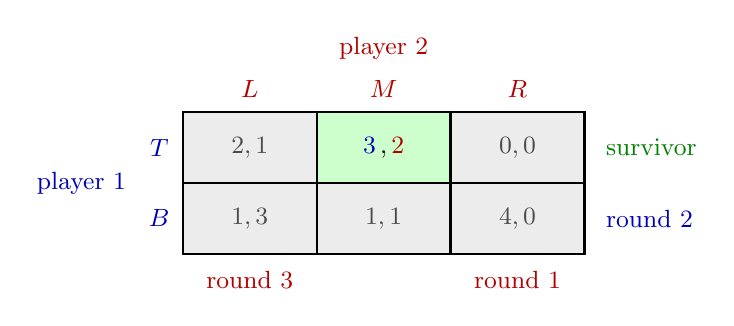
\begin{tikzpicture}[font=\small, >={Latex[length=2mm]}]
  \def\w{1.7} \def\h{0.9}
  % shading: deleted cells grey, survivor green
  \fill[gray!15] (0,-\h) rectangle (3*\w,0);
  \fill[gray!15] (0,0) rectangle (\w,\h);
  \fill[gray!15] (2*\w,0) rectangle (3*\w,\h);
  \fill[green!20] (\w,0) rectangle (2*\w,\h);
  % grid
  \draw[thick] (0,-\h) rectangle (3*\w,\h);
  \draw[thick] (\w,-\h) -- (\w,\h);
  \draw[thick] (2*\w,-\h) -- (2*\w,\h);
  \draw[thick] (0,0) -- (3*\w,0);
  % strategy labels
  \node[red!70!black] at (0.5*\w,\h+0.3) {$L$};
  \node[red!70!black] at (1.5*\w,\h+0.3) {$M$};
  \node[red!70!black] at (2.5*\w,\h+0.3) {$R$};
  \node[blue!70!black] at (-0.3,0.5*\h) {$T$};
  \node[blue!70!black] at (-0.3,-0.5*\h) {$B$};
  \node[red!70!black, anchor=south] at (1.5*\w,\h+0.55) {player 2};
  \node[blue!70!black, anchor=east] at (-0.6,0) {player 1};
  % payoffs
  \node[gray!60!black] at (0.5*\w,0.5*\h) {$2,1$};
  \node at (1.5*\w,0.5*\h) {\textcolor{blue!70!black}{$3$}\,,\,\textcolor{red!70!black}{$2$}};
  \node[gray!60!black] at (2.5*\w,0.5*\h) {$0,0$};
  \node[gray!60!black] at (0.5*\w,-0.5*\h) {$1,3$};
  \node[gray!60!black] at (1.5*\w,-0.5*\h) {$1,1$};
  \node[gray!60!black] at (2.5*\w,-0.5*\h) {$4,0$};
  % deletion order
  \node[red!70!black, anchor=north] at (2.5*\w,-\h-0.1) {round 1};
  \node[blue!70!black, anchor=west] at (3*\w+0.15,-0.5*\h) {round 2};
  \node[red!70!black, anchor=north] at (0.5*\w,-\h-0.1) {round 3};
  \node[green!50!black, anchor=west] at (3*\w+0.15,0.5*\h) {survivor};
\end{tikzpicture}
\end{document}
